\section{Mekong}

26 juin 2008

\begin{multicols}{2}

Mékong, Mékong... ça me dit quelque chose...

Mais oui c'est bien ça, le fleuve qui part de Chine, fait la frontière entre la Thaïlande et le Laos puis va au Cambodge. Je suis parti de Pai en bus direction Chiang Khong, ville Thai faisant face a Huay Xay, ville Laotienne. C'est donc là que j'ai passé les deux postes d'émigration et d'immigration, puis je me suis enbarqué sur un bateau pour descendre sur le Mékong vers Luang Prabang, en deux jours.

Pour cet article, exceptionnelement je ne vous propose que des photos, en effet le recit de ces deux jours tient en deux mot : chill out.

%\hspace*{-0.65cm}
%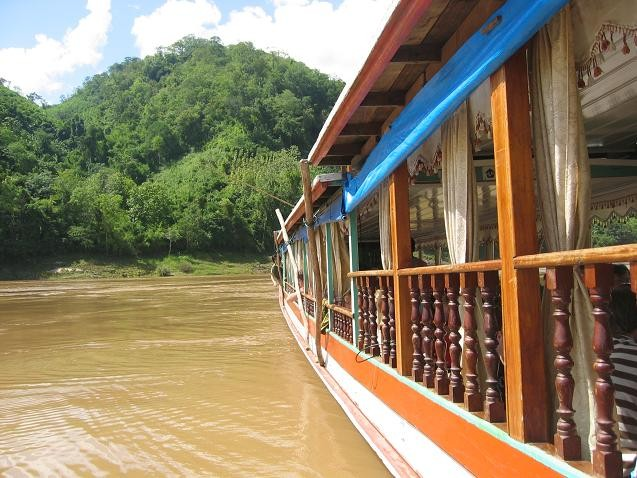
\includegraphics[width=4.8cm]{articles/Mekong/1214473370zy1a.jpg}
%Le bateau vu en longueur.

%\hspace*{-0.65cm}
%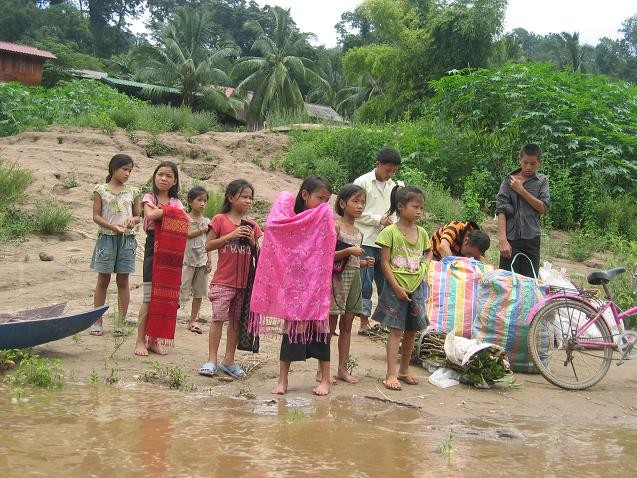
\includegraphics[width=4.8cm]{articles/Mekong/12144733896AMi.jpg}
%Des enfants sur la berge.

%\hspace*{-0.65cm}
%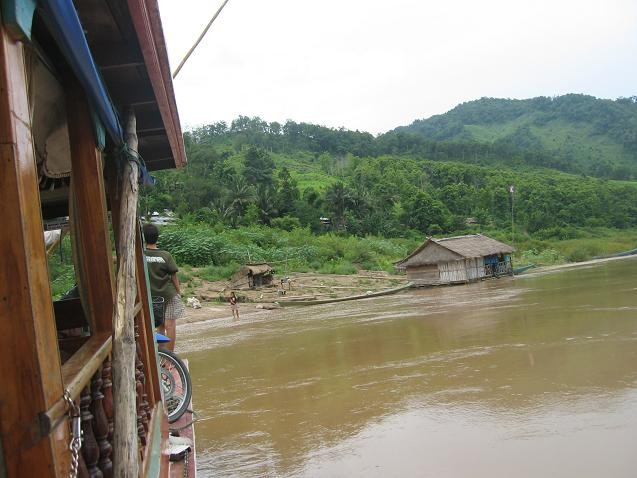
\includegraphics[width=4.8cm]{articles/Mekong/1214473395mtro.jpg}
%Encore une escale.

%\hspace*{-0.65cm}
%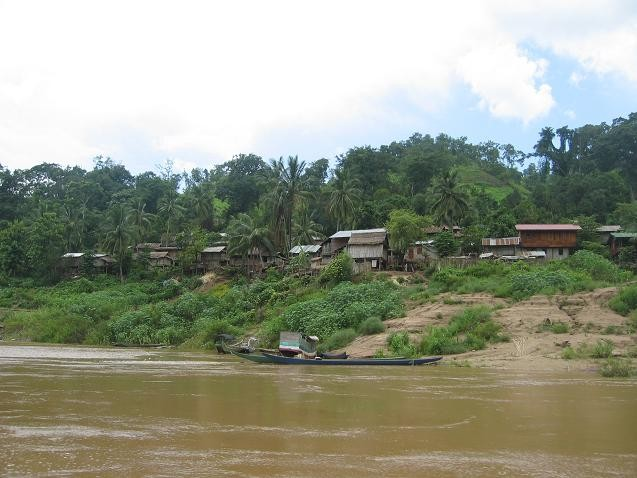
\includegraphics[width=4.8cm]{articles/Mekong/1214473400ezNu.jpg}
%Un village sur la côte.

%\hspace*{-0.65cm}
%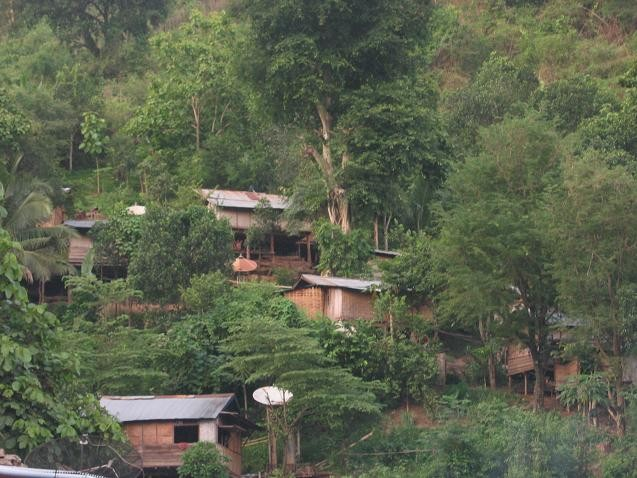
\includegraphics[width=4.8cm]{articles/Mekong/1214473407uNUm.jpg}
%Escale du soir.

\end{multicols}

\bigskip
\textbf{\textsc{Commentaires}}

\medskip
Titou a écrit le 13 juil. 2008 :
\begin{displayquote}
Eh ti dud !
Bon je voulais juste mettre un petit post sur ton blog pour ne pas laisser ce blanc tout pas beau en bas de ton message! Profites bien de tes derniers jours et je te dis à très bientôt !
Biz mon pote
\end{displayquote}

\medskip
Helene et Dova a écrit le 14 juil. 2008 :
\begin{displayquote}
Coucou Etienne!
Alors content de retrouver ta petite ile indonesienne :-)?
Nous venons de naviguer sur ton blog, et nous n'avons pas trouve de photos recentes. Aurais tu d'autres choses plus interessantes a faire?
Nous attendons toujours avec impatience les photos de Vang Vieng.
Aussi, nous n'avons pas ton e-mail.
Quand repars tu de Bali? Nous Arrivons le 23.
A bientot la bas, par mail ou mieux encore a Paris.
Cheers Helene \& Dova
\end{displayquote}

\medskip
Helene \& Dovaline a écrit le 11 sept. 2008 :
\begin{displayquote}
Hola guapo!!!
Alors tu te fais a la vie parisienne? La ligne 2, c'est quoi ça??? Nous avons décidé d'effacer tous les mauvais souvenirs. Nous ne voulons meme pas penser au retour a Paris et d'ailleurs on se demande si on va vraiment rentrer.
Nous sommes actuellement au Chili, a Valparaiso. Demain nous partons pour le Nord. Nous remontons lentement ce pays avant de rejoindre la Bolivie et le Perou. Ici il fait froid, on a du se refaire au plus vite une garde-robe. Lávantage c que nous avons a notre grande surprise pu skier a seulement 42 kms de Santiago... Grandiose et grand ciel bleu. Faudra aller voir les photos sur le blog.
Envoie nous ton mail perso sur notre adresse mail stp et aussi nous sommes impatientes d'enfin voir les photos de Vang Vieng.
A bientôt mais pas trop tôt car on encore soif de decouverte.
Muchos besos
Helene \& Dova
\end{displayquote}

